 \documentclass[onecolumn,11pt]{article}
%*********
%Paquetes
%*********
\usepackage[spanish]{babel}
\usepackage[utf8]{inputenc}
\usepackage[a4paper, total={7in, 9in}]{geometry}
\usepackage{amsfonts}
\usepackage{dsfont}
\usepackage{physics}
\usepackage{xcolor}
\usepackage{tikz-cd} %para diagrama conmutatitvo
\usepackage{multicol} %para la lista de operadores
\usepackage{hyperref}
\usepackage{caption}
\usepackage{subcaption} %para las subfiguras
\title{SWAP efectivo}
\date{\today}
%*********
%Comandos
%*********
\newcommand{\mcU}{\mathcal{U}}
\newcommand{\mcO}{\mathcal{O}}
\newcommand{\mcI}{\mathcal{I}}
\newcommand{\mcL}{\mathcal{L}}
\newcommand{\mcS}{\mathcal{S}}
\newcommand{\hilbert}{{\sf H}}
\newcommand{\mcB}{\mathcal{B}}
\newcommand{\mcH}{\mathcal{H}}
\newcommand{\mcF}{\mathcal{F}}
\newcommand{\mcC}{\mathcal{C}}
\newcommand{\mcT}{\mathcal{T}}
\newcommand{\mcE}{\ensuremath{\mathcal{E}} }
\newcommand{\mcG}{\ensuremath{\mathcal{G}} }
\newcommand{\mcM}{\mathcal{M}}
\newcommand{\mcN}{\mathcal{N}}
\newcommand{\nnn}{\mathcal{N}}
\newcommand{\choi}{\ensuremath{\mcD} }
\newcommand{\mmm}{\mathcal{M}}
\newcommand{\sss}{\mathcal{S}}
\newcommand{\mcD}{\mathcal{D}}
\newcommand{\mcA}{\mathcal{A}}
\newcommand{\mcP}{\mathcal{P}}
\newcommand{\Complex}{\mathbb{C}} %Para escribir al espacio de hilbert complejo
\newcommand{\Id}{\mathds{1}}% Para escribir el op. indentidad con notación chida
\newcommand{\CG}[1]{\mcC\left[#1\right]}
\newcommand{\Fuzzy}[1]{\mcF\left[#1\right]}
\newcommand{\nota}[1]{{\color{red} [#1]}}
\newcommand{\notaAd}[1]{{\color{blue} [#1]}} %Notas pero mías

\begin{document}
\maketitle
\thispagestyle{empty}
EL objetivo de esta tarea era ver si un conjunto se mostraba invariante bajo un SWAP subyacente\cite{CGEmergingDynamics}.
\section{Unitaria}

Una operador unitario se traduce como una rotación en la esfera de Bloch. Entonces dos operadores están relacionados por una unitaria si sus vectores de Bloch tienen la misma norma (esto es, los operadores tienen la misma norma de Frobenius).

Si consideramos un estado sobre el eje z,

\begin{equation}
\rho_{z}=\frac{1}{2}\qty(\Id+z\sigma_{z})
\end{equation}

entonces este está relacionado mediante a una unitaria a cualquier estado $\rho$ con vector de Bloch $\vec{r}$ tal que $\abs{\vec{r}}=z$.

\section{Mapeo de asignación}

Sea $\rho_{z}$ un estado grueso sobre z definido como antes, y sea $\{\psi_{i}\}_{i=1}^{N}$ el conjunto de estados con los que se obtiene su estado fino asignado. Además, sea $\rho$ un estado grueso tal que $\abs{\vec{r}}=z$.

\begin{equation}
\Rightarrow \exists U \text{ tal que } U\rho_{z}U^{\dag}=\rho
\end{equation}

Sea $\mcU=U\otimes U$, $\sigma_{i}'=U\sigma_{i}U^{\dag}$. En las siguientes líneas se muestra que si se rota a todo el conjunto $\{\psi_{i}\}$ usando $\mcU$, lo que se halla es el conjunto fino para el mapeo de asignación de $\rho$.

\notaAd{Aquí estoy asumiendo que rotar a todo el conjunto mantiene la medida de Haar. Con esto me refiero a que el conjunto rotado sigue teniendo una distrubución bonita que permita sacar un promedio decente.}

\begin{align*}
\CG{\mcU \psi_{i} \mcU^{\dag}}=&\Tr_{2}\qty[p\mcU\psi_{i}\mcU^{\dag}+(1-p)\mcU S \psi_{i} S^{\dag}\mcU^{\dag}]\\
=&\Tr_{2}\qty[p\mcU\qty(\frac{1}{4}\sum_{i,j}\gamma_{ij} \sigma_i\otimes\sigma_j)\mcU^{\dag}+(1-p)\mcU S \qty(\frac{1}{4}\sum_{i,j}\gamma_{ij} \sigma_i\otimes\sigma_j) S^{\dag}\mcU^{\dag}]\\
=&\Tr_{2}\qty[p\mcU\qty(\frac{1}{4}\sum_{i,j}\gamma_{ij} \sigma_i\otimes\sigma_j)\mcU^{\dag}+(1-p)\mcU \qty(\frac{1}{4}\sum_{i,j}\gamma_{ij} \sigma_j\otimes\sigma_i)\mcU^{\dag}]\\
=&\Tr_{2}\qty[p\qty(\frac{1}{4}\sum_{i,j}\gamma_{ij} \sigma_{i}'\otimes\sigma_{j}')+(1-p)\qty(\frac{1}{4}\sum_{i,j}\gamma_{ij} \sigma_{j}'´\otimes\sigma_{i}')]\\
=&\frac{1}{2}\qty[\Id +p\sum_{i=1}\gamma_{i,0}\sigma_{i}'+(1-p)\sum_{j=1}\gamma_{0,j}\sigma_{j}']\\
=&\frac{1}{2}\qty[\Id + \sum_{i=1}^3[p\gamma_{i,0}+(1-p)\gamma_{0,i}]U\sigma_{i}U^{\dag}]\\
=&U\frac{1}{2}\qty[\Id + \sum_{i=1}^3[p\gamma_{i,0}+(1-p)\gamma_{0,i}]\sigma_{i}]U^{\dag}\\
=&U\CG{\psi_{i}}U^{\dag}\\
=&U\rho_{z}U^{\dag}\\
=&\rho
\end{align*}
Como esto es para todo $i$, si se rota cada $\psi_{i}$, lo que obtenemos es un conjunto que podemos promediar para hallar el estado fino asignado a $\rho$. Aún mejor, como el promedio es lineal:
\begin{align}
\mcA[\rho]=&\frac{1}{N}\sum_{i}U\psi_{i}U^{\dag}\\
=&U\qty(\frac{1}{N}\sum_{i}\psi_{i})U^{\dag}\\
=&U\mcA[\rho_{z}]U^{\dag}
\end{align}
Esto significa que podemos hallar el mapeo de asignamiento de un estado $\rho$ a través del mapeo de asignamiento de otro estado $\rho_{z}$, siempre y cuando exista una unitaria entre estos.


\section{Numérica}
\subsection{Cascarón de estados mixtos}
Se generan estados puros $\begin{pmatrix}
a\\
b\\ \end{pmatrix}$ de manera uniforme. Estos son puntos en el cascarón unitario. Todos estos puntos se deplazan radialmente hacia adentro mediante un factor:
\begin{equation}
\vec{\alpha}=r\vec{\alpha_{0}}
\end{equation}
El resultado es un conjunto de estados mixtos $\{\rho_{i}\}_{i=1}^{N}$ cuyos vectores de Bloch se encuentran en el cascarón de radio $r$.

\subsection{Mapeo de asignación para el cascarón}


A cada $\rho_{i}$ hay que hallarle su estado fino asignado. Lo que se hace es generar un conjunto $\{\psi_{i}\}_{i=1}^{N}$ de estados finos para un estado grueso en $z$, $\rho_{z}$, tal que su coordenada en $z$ es justamente el radio del cascarón.

Como existe una unitaria $U_{i}$ entre $\rho_{z}$ y cada estado de $\{\rho_{i}\}_{i=1}^{N}$. Entonces podemos aplicar estas unitarias para hallar todos los $\mcA[\rho_{i}]$.

\subsection{Resultados}

Dos experimentos. En el primero se utiliza una probabilidad de swap $p=0.5$ (cascarón de radio $r=0.3$). El conjunto no cambia. En el segundo se utiliza una probabilidad de swap $p=0.3$ (cascarón de radio $r=0.8$).

Se grafican dichos cascarones en azul. Se aplica un SWAP a todos los $\mcA[\rho_{i}]$, y se saca el coarse graining. El resultado se grafica en amarillo.

\begin{figure}[h]
\centering
\begin{subfigure}{0.4\textwidth}
  \centering
  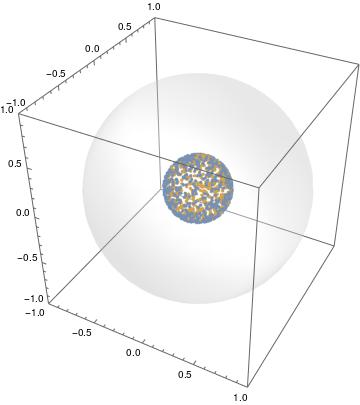
\includegraphics[width=0.8\linewidth]{figures/effectiveswap_p=0.5_z=0.3.jpeg}
  \caption{$p=0.5$, $r=0.3$, el conjunto no cambia después del swap subyacente}
  \label{fig:paralelogram}
\end{subfigure}
\begin{subfigure}{0.4\textwidth}
  \centering
  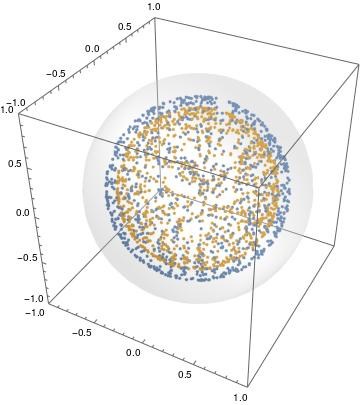
\includegraphics[width=0.8\linewidth]{figures/effectiveswap_p=0.3_z=0.8.jpeg}
  \caption{$p=0.5$, $r=0.3$, el conjunto se contrae  después del swap subyacente}
  \label{fig:paralelogram}
\end{subfigure}
\label{fig:cooldensities}
\end{figure}
\bibliographystyle{ieeetr}
\bibliography{bibliography}


\end{document}
